\chapter{Introduction}
\label{ch01}
\mquote{Computations across mappings are called transformations.}{J. Greenfield, K. Short, S. Cook, S. Kent, Software Factories, Willey, 2004}

%Those
%luminous curves, where the shadows have a golden tone, that tissue as
%firm as a sinew and as \textit{mobile} as the most delicate membrane, is a
%crowning achievement of nature. - Scenes from a Courtesan's Life, Honor\'e de Balzac, gutenberg.org

\noindent \textit{Attribute Enabled Programming} (AEP) is a wide-spreading technique that uses explicit attributes \cite{java.explicit.programming} directly in the programming language level to decorate code existing entities, in order to modify their semantics. AEP is supported in several general purpose languages, such as .NET (attributes) \cite{csh.attrib}, or Java (annotations) \cite{www.java.meta}. AEP is also supported by modeling languages, such MOF, UML (tagged values, stereotypes) \cite{www.mof}. AEP enables developers to enhance the semantics of an existing language with embedded domain specific language constructs, without any need to change the language grammar. Developers can use AEP to customize a language to fit their needs, without having to worry about parsing and grammar rules.

AEP is not a mainstream methodology, rather it complements ubiquitously existing programming methodologies. It can be appended in the top of any existing programming model (methodology), such as, \textit{object-oriented programming} (OOP), or \textit{aspect-oriented programming} (AOP) \cite{kiczalesetal.97}. Hence, the name Attribute Enabled Programming is preferred, and not something else, such as, Attribute Oriented Programming.

As AEP becomes more widely used, it can be easily overused and attribute annotations may fail to scale. Attributes are very easy to introduce, and depending on the automation associated with them, cheap to process. This could result in a large number of attributes used in unstructured ways within a project, or, in the general case, within a product-line made up of several related projects. The interpretation of many inter-related attributes could also become a bottleneck. Attribute dependencies further complicate the interpretation and add-hoc programming solutions cannot scale. A well defined development methodology that covers all the steps of \textit{Attribute Enabled Software Development} (AESD) needs to be applied.

This book addresses AESD for mobile software applications and shows that a software abstraction, called attribute-supported generative container, when directly supported at the programming language level, provides an effective means to automate the development of product-line software that runs on mobile devices.
This chapter presents the book in a nutshell. The need to automate the development of software for mobile devices is motivated by its role, extensive spread, and ever increasing complexity, in a world of ubiquitous computing. A short overview of the current technology for automation in the domain of mobile software is presented, justifying the need for advancing the technology, followed by a high-level presentation of the proposed technology. The chapter ends with a brief overview of the contribution of this book and with a preview of its structure.

%In this work, we deal with transformation techniques at the programming language level, to support product-line automation of mobile software in the context of ubiquitous computing, using a declarative attribute-based generative container abstraction.

\section{Mobile Software in a Ubiquitous Computing World}

The term \textit{ubiquitous computing} (\textit{ubicom} for short) was first coined in the beginning of the '90s in a series of articles by Mark Weiser \cite{Weiser.01,Weiser.02,Weiser.03}, while he was heading the Computer Science Laboratory at Xerox PARC. Ubiquitous means present or found everywhere, i.e., omnipresent\footnote{All definitions are based on Oxford English Dictionary (OED), \url{http://dictionary.oed.com}}, and implies transparency, i.e., the interaction with the computers is not explicit anymore. Computers become an integral part of the entire environment. Weiser says that \textit{"The most profound technologies are those that disappear. They weave themselves into the fabric of everyday life until they are indistinguishable from it."} \cite{Weiser.01}.

The ubiquitous computing ideas have emerged from the observation that the technology is becoming mature and cheap enough to be multiplied widely in the environment. The computer hardware is becoming less expensive and its size smaller as the number of transistors per chip grows. It could be afforded to have many specialized computers around: \textit{"Ubiquitous computers will also come in different sizes, each suited to a particular task."} \cite{Weiser.01}. %Ubiquitous computing is an engineering problem. It is about finding new ways to combine technology and to optimize it to serve specific problems. Control systems spread in the environment\footnote{Environment - The overall physical, systematic, or logical structure within which something operates. (OED)} with rich interactive interfaces are now being a matter of willingness, not of technology. Magical devices and objects that serve us are part of our imagination from the start of time, when humans learned to create tools and profit by using them. The technology development is used to fulfill this imagination.

The current trend of ubiquitous computing ideas is often labeled by the term \textit{ambient intelligence} (AmI) \cite{AmI,ami2003}, technically defined as a combination of \textit{"Ubiquitous Computing, Ubiquitous Communication and Intelligent User Interfaces"} \cite{AmI}. The \textit{ambient} is the surrounding environment and often the term is used interchangeably with \textit{environment}. While ubiquitous computing means more than one computer, ubiquitous communication means that computers do not live in isolation, but somehow communicate with each-other. Intelligent user interfaces stand for personalized interaction with a ubiquitous computing environment in natural human ways, such as, voice (speech), or gestures. AmI is about combining different technologies toward a visionary goal, to enable various services and properties that the surrounding environment should have.

\noindent Ubiquitous computing has also been treated as a combination of:
\begin{itemize}
\item \textit{natural interfaces}, another name for implicit and transparent human-computer interfaces, 
\item \textit{context-aware applications}, related to the location, object identity, time history, user identification, etc. (who, what, where, when, why),
\item  \textit{automated capture and access systems}, that enable recording and finding live experiences, e.g., meeting notes, and 
\item \textit{everyday computing}, that addresses ubiquitous tasks that have a continuous timespan with no known end and that span through various concurrent activities \cite{tochi-millenium}. 
\end{itemize}
%\subsection{Pervasive and Mobile}

\noindent There are two ways (\fig{fig:ch01pm}) which can be used in isolation but more often in combination to implement ubicom scenarios:

\begin{figure}[ht]
	\begin{center}
		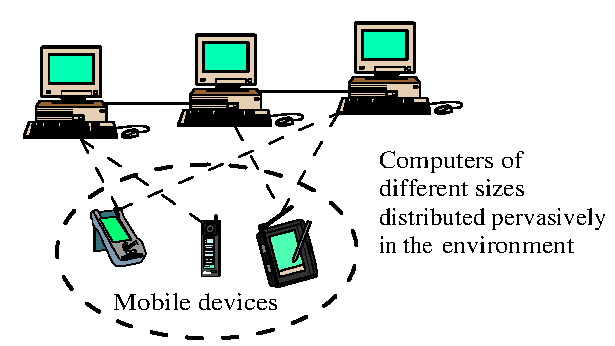
\includegraphics[width=7cm,height=!]{ch01/pm}
	\end{center}
	\caption{Pervasive and Mobile Devices}
	\label{fig:ch01pm}
\end{figure}

\begin{enumerate}[a.]

\item The technology can be \textit{pervasive}, that is, the computers are extended and diffused throughout every part of the environment. In a pervasive environment, the computational resources will tend to be uniformly distributed among the objects. The objects will contain a combination of sensors, and / or \textit{embedded} computers, and communication capabilities with humans (interface) or other computers. The objects will look like autonomous individuals, and every object will have its own processing unit, where it autonomously keeps track of the surrounding environment. That is, each object should have its own computer, its own sensors, and its own (unique) ways to communicate with and affect the rest of the environment. Depending on the context \cite{schilit94contextaware}, that is, the object location in the environment \cite{hightower01survey}, each object will create its own unique understanding of the environment and its history, and decide how to affect the environment in the future. In practice, some global view of the environment, along with the distribution of computational resources, makes it possible to optimize the coordination of object reactions (better context management). At present, it is also cheaper and easier to spread only sensors and the communication hardware, e.g., using the \textit{smart dust} technology \cite{kahn99next,warneke01smart}, and keep some of the event processing centralized.

\item The technology can be \textit{mobile}, that is, not stationary but movable around the environment, usually in the form of a personal computing device, or a \textit{wearable} computer \cite{wearable.1998}. It is the interaction with a ubicom environment, where the \textit{mobile} view of the technology becomes important. Suitable forms of interaction are needed to control a ubicom environment \cite{tochi-millenium}. Computers create a virtual model of the environment and operate in this model. The real world events should be converted to this virtual model, used to modify the state of the virtual model, and then the virtual model changes should be converted back to events than affect the real world. Human communication with a ubicom environment is part of this translation of the real world events.

Mobile devices offer convenient and suitable ways to map human interactions in a ubiquitous environment and are often an integral part of ubicom scenarios. Using a mobile device is simpler that moving to reach a touch screen nearby. There is no need to stay in a queue to use a mobile device, as it would be the case with a shared device when there are other people in the same place. Using mobile devices for interaction, also does not conflict with using other forms of communication, e.g., voice and gestures, but can be used to augment them.
%
There are also several other reasons why mobile computing and mobile applications are important for achieving ubiquitous computing. 

The non-uniform distribution of technology is likely to prevail. Not all environments will be equipped in the same ways. A mobile device that people can carry with, is a constant factor to rely upon, when designing applications in a non-uniform ubicom environment. It is cheaper to carry the technology around (e.g., a mobile phone), rather than replicate it in every corner (e.g., a public telephone cell every two meters). Even if a completely pervasive view of technology becomes possible and uniformly distributed, the mobile alternative pollutes the environment less with technology. Last but not least, a mobile device is a form of personal possession that can be carried always with. It may be used even if no networking is present. It makes sense to store data in a mobile device which are very personal, but difficult to remember, e.g., encrypted lists of passwords, financial records, and software that may be continuously needed.

Mobile phones were the first mobile devices to have global success and wide acceptance. Based on this success, there is a trend to enrich the number of services that are offered to people via mobile phones, benefiting from an extensive existing user base. The demand for more functionality is followed by a competitive supply of better hardware \cite{j2me.2005} and software for mobile devices. 
Mobile phones and mobile computers (Personal Device Assistants - PDAs) are becoming more powerful for less physical space. Both classes of devices are converging to a single device that has a telecommunication (networking) function and also serves as a personal computer device. This has opened a profitable market for third-party software for mobile devices supported by several platforms, e.g., J2ME \cite{www.j2me}, .NET CF \cite{dnetcf}, and BREW \cite{brew}, as well as frameworks \cite{ubi.infra.survey}, followed by a need for more applications that should be delivered in time. 

\end{enumerate}

%\subsection{Product-Lines for Mobile Device Software}
% The increasingly powerful mobile devices raise the need for more software specialized and optimized to run on them. It may seem that the restrictions in the processing power and other characteristic capabilities that mobile devices have currently, compared to desktop computers, are only temporary. However, there will be always restrictions on what can be done with a mobile device, compared to other more powerful contemporary devices, e.g., desktop PC-s.  

\section{Automating Mobile Software Development}

Mobile devices and their applications play an important and increasing role in ubiquitous computing. There are several non-functional ubicom challenges \cite{design.ubicom.2002} related to software infrastructure, e.g., the way to build and organize the application functionality, seamless migration of logic among devices and different environments, device software modeling, and scalability of the solutions.
To address these issues, the status of mobile software development needs to change from a craft, employed in a case by case manner, to a fully automated \textit{product-line} specialized for mobile applications. A product-line offers the possibility to reuse in the future the common investment done in a series of individual products \cite{Parnas.pl.96,pl.02}.

Mobile device applications share a lot of common non-functional features, e.g., screen management and data persistence\footnote{Preservation of the data, this is, the ability to store and load back the stored data.}, that can be factored out and made part of an automated product-line. The common functionality can then be requested declaratively and injected automatically in particular mobile device applications. Maximum automation can be achieved by focusing on a mobile application domain, and developing technology that takes into consideration the specific characteristics of the domain\footnote{A \textit{domain} is a specialized body of knowledge, an area of expertise, or a collection of related functionality \cite{pl.02}.}. Mobile applications are easier to automate than their desktop or server counterparts, because they have limited variability, e.g., in the ways the user interface is composed, or in the possibilities available for data persistence. Despite the advances in hardware technology, there is a set of properties that remain specific for mobile software, e.g., the limited screen size, low memory usage, sporadic networking, and ease of use, that need to be specially addressed. 

\begin{figure}[ht]
	\begin{center}
		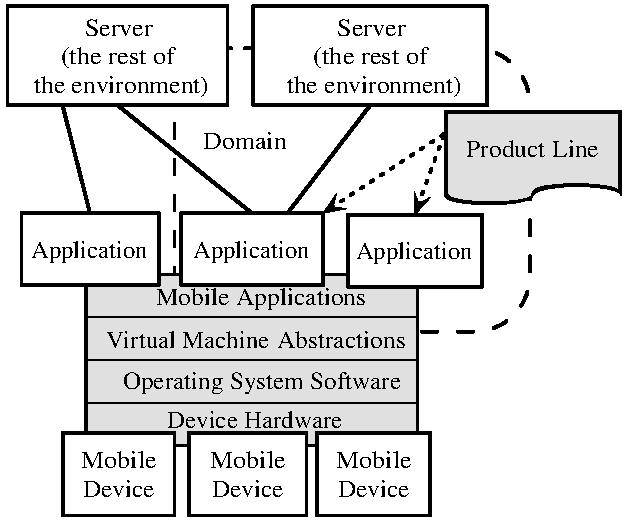
\includegraphics[width=10cm,height=!]{ch01/mobiledomain}
	\end{center}
	\caption{Mobile Device Applications Domain}
	\label{fig:ch01domain}
\end{figure}

At the software application level, isolation from specific mobile device hardware and specific operating system software can be achieved by using virtual machine abstractions, e.g., J2ME Mobile Information Device Profile (MIDP) \cite{www.j2me} and .NET Compact Framework \cite{dnetcf}. The focus in this book is in the domain of mobile applications that run on mobile devices supported by \textit{virtual machine} abstractions (\fig{fig:ch01domain}). As shown in \fig{fig:ch01domain}, several related mobile device applications can be managed by a product-line that addresses common repetitive technical issues. In a ubiquitous environment a mobile application also communicates with the environment as a client of one or more services, e.g., to access data in a central server-side location. Part of the server-side software found in the environment is closely related to the functionality of mobile device applications and may not be needed for other types of clients. This server-side part is represented inside the dashed box in \fig{fig:ch01domain}. It contains also repetitive technical concerns that need to be addressed by the product-line. A systematic and automatic approach for mobile application software development that addresses both client- and server-side issues is required. 

\subsection{Programming Models for Mobile Software}
\label{mobile.models}

Mobile and especially embedded software has been always difficult to write and debug for several reasons. There is a gap between the machine where the software is developed, usually a desktop PC machine, and the actual device on which the software will run. This gap requires using various emulators for the actual devices in order to build and test the actual software. One more step, namely emulator testing and (remote) debugging, is added to the usual development cycle of desktop software. Various implicit coding conversions, based on the language or specific API\footnote{Application Programming Interface.} restrictions, must also be followed in order to write efficient software.

\begin{figure}[ht]
	\begin{center}
		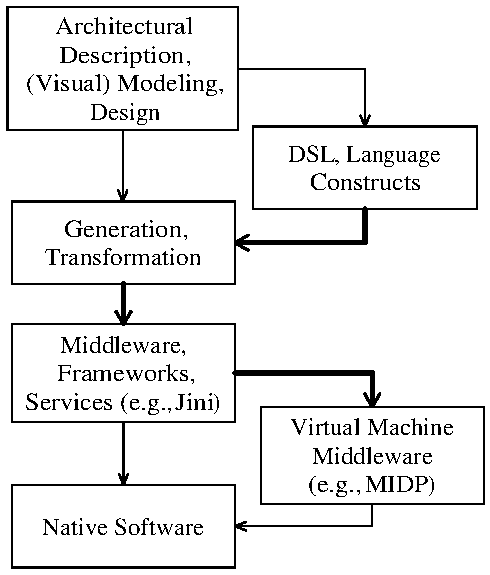
\includegraphics[width=7cm,height=!]{ch02/pm}
	\end{center}
	\caption{Programming Models for Mobile Software}
	\label{fig:pm}
\end{figure}

\fig{fig:pm} shows a high-level view of the common techniques used to develop software for small devices, such as, visual modeling and domain-specific languages (DSL) \cite{deursenetal.00}. Programming small devices can start at any node of the diagram in \fig{fig:pm}. Not all systems use all the paths shown, and more than one path is possible. For example, the model of an application can be defined by using visual domain abstractions. This visual model is then either converted to a specific DSL, or is used to generate directly source code in a general-purpose language. The generated code targets directly the native software, or makes use of existing middleware frameworks. The application could run against the device hardware, or on the top of a virtual machine. Various forms of these programming models have been used in real-time embedded systems \cite{realtime.77,ghosh94survey,emb.gen.02}, and other embedded software and frameworks \cite{BurchPasseroneSangiovanni-Vincentelli2001,emb.comp.03}.

Mobile device applications addressed in this book have less restrictive requirements than embedded systems, but more restrictions than other PC desktop software. Virtual machines, e.g., J2ME \cite{www.j2me}, .NET CF \cite{dnetcf}, and their programming models, such as MIDP \cite{www.midp-ota}, help to hide the hardware and software details for different classes of mobile devices. Virtual machines, however, do not offer high-level abstractions for application domains. As the focus on ubiquitous computing grows, so does the number of mobile applications that need to be developed and debugged. There are more and more applications for mobile devices that share a lot of similarities, but also have their own peculiarities. Reusing only the virtual machine abstractions to hide OEM\footnote{Original Equipment Manufacturer.} specific device details is not sufficient any more. The commonality and variability of families of applications must be supported as well.

More than one programming abstraction of \fig{fig:pm}, e.g., visual modeling, DSL and code generation, can be used to factor out and reuse the common functionality, and some of them are more declarative than the others. The approach presented in this book goes along the bold connection lines in the \fig{fig:pm}. The goal is not to develop a new kind of middleware system, but rather to propose ways that automate the creation of third-party mobile software by relying on existing middleware, such as MIDP \cite{www.midp-ota}. MIDP application development can be supported with abstractions that organize and reuse MIDP specific domain functionality. The interest will be in declarative representation of the domain abstractions at the source code level. Declarative constructs preserve the domain abstractions in the source code, and reduce the development and debugging time by hiding the details of a more complex underlying programming model.

\subsection{Variation Mechanisms for Mobile Application Product-Lines}

There are different ways to parameterize the common behavior characterizing a domain and reuse it in a specific application, known also as \textit{variation mechanisms} \cite{pl.00}. The automation of mobile device software product-lines requires generic software technology to support \textit{iterative} \see{sec.iterative.pl} product-line development. This means that the variation mechanisms should be:
\begin{enumerate}[a.]
\item Easy to introduce and maintain (low-cost). The iterative development of a product-line is important to support product-line evolution \cite{Pussinen.2002}.  
\item Flexible to support design experimentation. The correct \textit{domain abstractions} used to represent the \textit{domain concerns} are often not completely known from the beginning and may change as the product-line evolves.
\item Declaratively supported to reduce accidental complexity \cite{brooks.87} and achieve transparent automation.
%
The domain dependent concerns should be injected automatically in a specific mobile application. Domain dependent concerns are code-related \textit{core assets} (reusable artifacts) for a domain \cite{pl.02}. 
\item Enable a clear separation of the common domain functionality and the application specific functionality and enable domain-specific optimizations. The domain concerns are usually \textit{cross-cutting} \cite{kiczalesetal.97}, that is, they are needed in more than one place (components) within an application.
\end{enumerate}

Several technologies \cite{pl.00} can be used to support variation, e.g., inheritance, component libraries (object-frameworks \cite{batoryetal.00}),
extensions (selection of variants), configuration,
parameterization, templates, macros,
generation \cite{generative.00},
(embedded) domain-specific languages (DSL) \cite{deursenetal.00}, compiler directives,
visual modeling and CASE\footnote{Computer Aided Software Engineering.} tools. All these variation mechanisms have their own benefits and drawbacks and need to be specifically evaluated for mobile software applications.
%
The library solution is the simplest one, as it requires no further tool support other than those offered by the development language. It offers minimal automation for inserting the domain concerns into an application. Code generation is easy to implement, but pure generative solutions\footnote{That is, generative techniques used alone, not in a combination with other variation mechanisms.} are difficult to maintain and debug because of the programming indirection and lack of early static checking.
DSL are more declarative and enable transparent automation, but have high start-up costs to be implemented. 
Visual modeling abstracts the domain concerns, but it does not support well iterative development of abstractions and traceability. Often it is not feasible to define every piece of behavior visually and source code artifacts are used instead\footnote{For example, a UML-based CASE tool may generate only code stubs, whereas the method internals need to be filled out manually. The functionality of the methods could also be specified visually, but unless the functionality is made of well-known repetitive code, it is often easier to program using source code directly.}. A more elaborated discussion of the variation mechanisms of interest for mobile product-lines is provided in \sr{c2sec:pline}.

\section{Attribute Enabled Software Development}

This book introduces variation mechanism that fulfills the requirements posed for mobile product-lines and does not have the problems encountered with other variability mechanisms. Mobile software product-lines can be implemented with programmable software container abstractions, backed up at the source code by lightweight domain-specific abstractions, encoded as explicit code attributes, which are interpreted by means of code transformation techniques. This section explains shortly what is meant by these terms.

\subsection{Mobile Containers}

A \textit{software container} is an architectural abstraction that can be used to organize a product-line for a domain, by factoring out the common domain behavior into a set of \textit{services} provided by the container. The container services are reused by all applications in the product-line. An application component inherits quasi-transparently the domain-wide features from the container it is deployed in. That is, when developing an application, the developer can focus exclusively on the features that are specific for the particular application at hand. The domain concerns are provided (\textit{injected}) when needed, into the components of the application by the container implementation. 

The container abstraction is known from enterprise server-side containers, e.g., COM+ \cite{comp.services} and EJB \cite{j2ee14}. The idea can be applied to organize services in every domain of interest, especially to achieve automation of a mobile product-line. The container creates a well-defined boundary between the domain abstractions and the rest of an application. For a mobile application, the container provides a single centralized point of maintenance, that wraps the underlying services offered by the middleware (e.g., J2ME \cite{www.j2me}), making it easier to support mobile software evolution.

\begin{figure}[ht]
	\begin{center}
		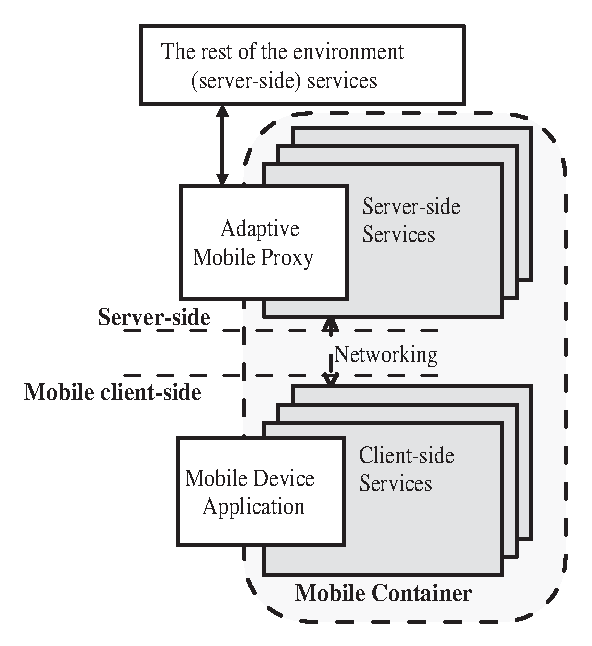
\includegraphics[width=8cm,height=!]{ch01/mobc}
	\end{center}
	\caption{Mobile Container Architecture}
	\label{fig:ch01mobc}
\end{figure}

The term \textit{mobile containers} will be used in this book to refer to a special combination of client and server containers which is appropriate to accommodate the specific characteristics of the domain of mobile applications. A mobile application is a client application with \textit{sporadic} network connectivity. As such, it is neither a thin nor a thick client\footnote{A thin client does only interface processing on the client-side and delegates any other data processing to the server-side. A thick client does most of the data processing on the client-side.}. It cannot be a thin client, because it should be able to do some processing and data storage on its own when disconnected. It cannot be a thick client either, because of the restricted resources of a mobile device. In order to save computing resources of the mobile device, as much of data processing as possible should happen on the server-side.

A distinction will be done between the server-side functionality that is specific for mobile device applications, and the functionality that is common for other types of clients\footnote{E.g., powerful desktop clients.}, as illustrated in \fig{fig:ch01mobc}. The server-side functionality that is common to mobile clients can be factored out from the rest of the server-side services in the form of an \textit{adaptive proxy} \cite{fox96adapting}. The mobile container is devised as a special kind of a software container \cite{server.patterns.02} that automates the organization and injection of domain concerns (a) in the mobile device client applications, shown in the lower part of \fig{fig:ch01mobc} and (b) in the intermediate application-level\footnote{Not to be confused with lower level proxies used to represent objects remotely over a network.} proxy part between the server (environment) services and the mobile clients. The adaptive proxy stands also on the server-side (\fig{fig:ch01mobc}). The server-part of a mobile container automates those aspects of the proxy that are directly connected with the functionality found on the mobile clients. It is the responsibility of the adaptive proxy to serve as a central connection point for representing the mobile clients and to communicate with the rest of the server-side services. The product-line handles the concerns of the both parts of the mobile container. 

To support the domain variability, the container itself should be \textit{programmable}, i.e., configurable, rather than providing a predefined set of services. The container can be used to inject any parameterized set of services into specific application components, using implicit or explicit architectural conventions. An open and extensible plug-in architecture with a configurable workflow is presented in this book \seec{ch05} to organize the product-line assets as container supported services. This enables software developers to specialize the product-line assets to fit their needs and to maintain them.

The inheritance of common properties from the environment is known as \textit{environmental acquisition} \cite{lorenz.96,ea.05} and could be supported by special language support. Some languages, e.g., Keris \cite{keris.04}, replace static linking with dynamic linking and can be used to support some form of environmental acquisition. The solution for modeling environmental acquisition presented in this book is \textit{lightweight} in the sense that, it can be  easily added to any existing language, making it suitable for iterative product-line development. The presented solution requires only a minimum extension to the existing language features, namely the ability to decorate the elements with attributes and support for interpreting the latter. The solution also makes the boundary between the application and the domain functionality explicit.

\subsection{Lightweight Domain-Specific Abstractions}

\textit{Domain-specific abstractions (DSA)} are language abstractions, usually in the form of embedded domain-specific languages (EDSL) \cite{kamin.98}, used to extend a general purpose programming language. DSA are used to add declarative support for specific concepts of a domain to a language, making it easer to write software for that specific domain. Having domain abstractions in code helps to preserve the domain architecture at the code level. The source code that contains the key abstractions of a domain declaratively is easier to understand. Declarative DSA blur the architectural gap \cite{sf.04} between a specific modeling step, and modeling directly at the source code level. DSA can be used to declaratively request the container-based services in the source code of a mobile application. As illustrated in \fig{fig:ch01dsaserv}, declarative DSA can be interpreted and automatically connected to the container provided services.


 %Thus, DSA reduce a step in debugging the final product-line code, rather than having, for example, to go though a visual modeling tool and refine the model. This is preferable, especially in the early stages of a product-line, when the final automation corresponding to the domain abstractions is not always quite clear. As the product-line development stabilizes, it is easy to introduce tool supported (visual) modeling for the domain based on the declarative DSA created.

\begin{figure}[ht]
	\begin{center}
		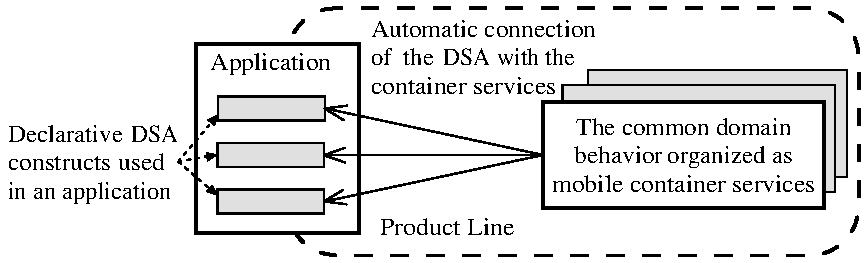
\includegraphics[width=12cm,height=!]{ch01/dsaserv}
	\end{center}
	\caption{Connecting DSA with the Container Services}
	\label{fig:ch01dsaserv}
\end{figure}

% Several abstractions may be needed to implement a container and to support its services. Such DSA should be easy to introduce and maintain.

Explicit attributes \cite{java.explicit.programming}, directly supported at language level, can be used as a low-cost mechanism to emulate DSA. Attributes\footnote{The terms \textit{attribute}, \textit{annotation}, and \textit{tag} will be used interchangeably to denote the same concept, unless explicitly noted otherwise.} are a lightweight language extension that remove the need to implement explicit domain specific language abstractions \cite{Taha.1997}. Attributes can be used as a variability mechanism to model product-line domain abstractions directly in the source code of a specific mobile application \see{attribute.families}. Attribute-based abstractions are cheap to introduce and to modify in a general-purpose language.
% and reduce the cost of introducing the domain abstractions.
 A language with support for attributes and attribute-driven transformations eliminates the need for other parsing and EDSL tools for implementing language abstractions to sustain mobile product-lines.

%The lightweight nature of attribute-based abstractions can be combined with generative \cite{generative.00} code techniques to enable domain-specific optimizations, for example to have a minimum level of abstraction layers. While attribute-based abstractions exist in the source code, they are treated as logical abstractions. That is, after attribute-based abstractions are interpreted / compiled, no further real abstraction layers are added to the system. For the programmer, however, the layers exist and could be used to reason about the system architecture of the domain.

Several general purpose language technologies, e.g., .NET \cite{www.dotnet} and Java \cite{www.java}, already offer some support for attributes. The main support provided by these technologies is to enrich structural entities, e.g., classes and methods, with attributes and to preserve such decorations in the binary meta-data\footnote{Data describing the other data.}. A more complete support for attributes and attribute transformations as part of the language technology is needed when attributes are used to emulate DSA. The abstract syntax tree (AST) created for the source code internally by the compiler, the AST-s created by various source processing tools (and API-s), and the AST obtained via reflection in languages that support meta-data, represent similar views of the same data structure, at various levels of detail\footnote{For example, the details of the method body are not modeled in the reflection API.}. The interfaces used to model these similar AST views are often different and the transformations done in one view are not easy portable to another view.

It is possible to unify all different AST representations, in a single data structure that provides support for different levels of detail. This generalized AST can be obtained either from source code or binary data, and can be used to implement attribute transformations for mobile product-lines. For attribute languages, this common representation will be called a \textit{Generalized and Annotated AST (GAAST)}, and the languages that offer such an API as part of their technology will be called \textit{GAAST languages}. The GAAST API, combined with ways to enable filtering nodes of interests, can be used as a common API to implement meta-programming attribute-driven transformations in a general-purpose language. If GAAST is part of the language, the investment on the transformation tools is protected as the language evolves.

Attribute enabled languages affect also the design \cite{design.attrib} process. OMG Model-Driven Architecture (MDA) \cite{mda.frankel} transformations, whose input models are represented as UML\footnote{Unified Modeling Language.} class diagrams, can be directly supported in a GAAST language. Using attributes to sustain DSA at the language level preserves architectural decisions of the domain models. GAAST languages require only type mappings to support several MDA Meta-Object Facility transformations. In MDA, the software development could start with a platform independent model (PIM), and then be iterated toward a platform specific model (PSM), introducing platform specific details in each step. GAAST languages offer a common API to directly support such transformations and open new possibilities to design applications, that will be investigated in detail in \kr{ch03}. 

\subsection{Attribute-Driven Transformations}

Any invasive \cite{java.compost} system that can access the abstract syntax tree (AST) of a program can be used to implement static attribute-driven transformations for attribute-based DSA in a product-line. For example, GAAST languages offer all the necessary means to support attribute-based transformations. The implementation of transformers in the GAAST API level is still very general, and may result in non-reusable transformers which are difficult to maintain.

Programming at the GAAST-level requires following implicit coding rules to be able to reuse the transformation behavior. Many AST manipulations based on the GAAST-API are repetitive across different transformation operations. Transformer implementations that directly build upon GAAST lack a clear structure of the transformation process. This opens the need for specialized transformer technology to enforce reusable modular organization of attribute-based transformers. Having modular transformers facilitates understanding the attribute semantics, and helps using attributes successfully to model the domain variability.

\begin{figure}[ht]
	\begin{center}
		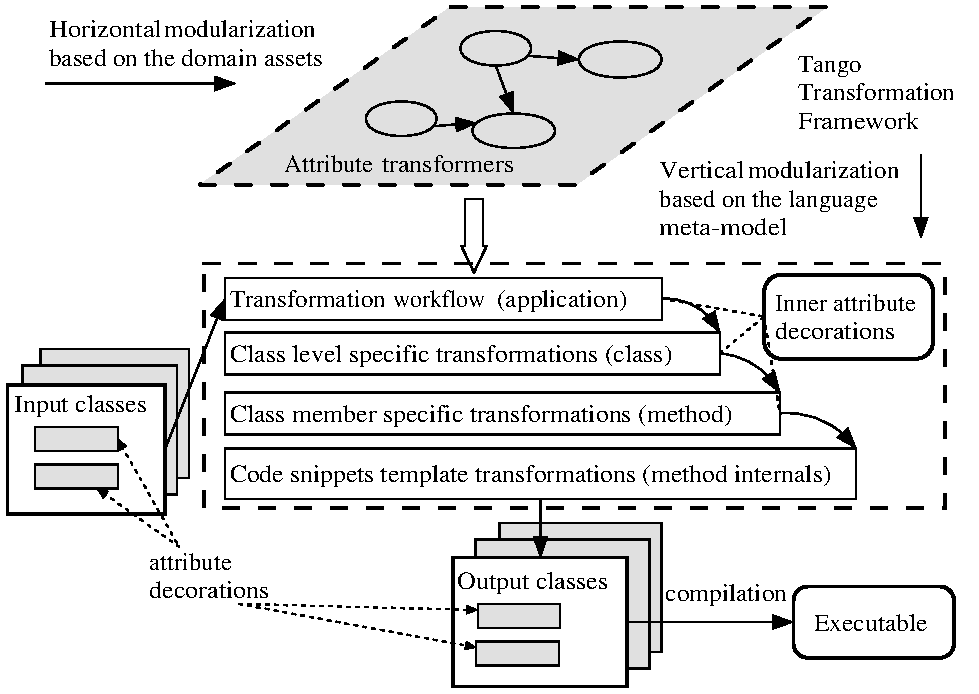
\includegraphics[width=15cm,height=!]{ch01/tango}
	\end{center}
	\caption{Layered Attribute-Driven Transformations}
	\label{fig:ch01tango}
\end{figure}

Knowledge about the domain, modeled as a set of attribute-based DSA, and about the deployed programming language can be explored to introduce a \textit{horizontal} and \textit{vertical} modularization for attribute-driven transformers (\fig{fig:ch01tango}). The transformation process can be structured horizontally according to the domain assets modeled with attribute-based DSA. The knowledge about the specific domain assets can be used to guide the transformation workflow. The workflow dependency graph can be partially computed automatically, based on local \textit{before} and \textit{after} dependency relations supplied by the developers that model the semantics of the interactions between the domain assets.

Knowledge about the structural nesting of the elements found in the language meta-model can be explored to organize the transformation strategy in vertical layers, as shown in the middle part of \fig{fig:ch01tango}. The approach for modular construction of attribute-based transformations taken in this book, embodied into the Tango transformation framework \seec{ch04}, supports a hardwired common OO language meta-model made of classes, fields, and methods, which in turn are made up of method code blocks. The hardwired meta-model enables a vertical layering that otherwise would not be possible with an arbitrary open meta-model. Some other frameworks \cite{stratego.01,www.aspectjt} deal with this issue by defining parameterized transformation operations, e.g., selection and iteration, that can work with any AST element type, but have a single layer to organize the transformation process. The approach presented in this book defines also declarative operations, but specializes them for each meta-model element type and organizes them in layers according to the language meta-model. The transformation process in Tango shown in \fig{fig:ch01tango} contains operations specialized for each transformation layer, e,g., class level specific operations. %This modularization can be automatically enforced.

%Splitting the transformation strategy allows to organize the transformer implementation into a series of layers. Each layer is only allowed to create transformers for elements of the lower layer, and delegates to them to carry out the exact details of the transformation. Furthermore, a layered transformation strategy enables reuse. The lower layer transformers focus in small atomic tasks and could be reused in more than one upper-level transformation. Organizing the transformation process in several stages \cite{Taha.1997} enables a high-level view of the transformation process and divides understanding what a transformer does at various levels of detail\footnote{Understanding what a transformer does often stops without the need to see what low-level layers do.}. Layering serves also to document the semantics of the set of attributes upon which a specific transformer works and helps to support transformation traceability.

Attribute-based transformers do not only operate on AST nodes that are explicitly decorated with attributes, they can also decorate the AST as they process it with \textit{inner attributes}, intended to support the transformation process (schematically shown in the middle right part of \fig{fig:ch01tango}). This technique is similar to saving the intermediate transformation results into declarative placeholders \cite{asfsdf.02}. Unlike in a compiler, where the AST decoration with attributes is used only internally \cite{java.compilers.book}, attribute-driven transformers treat the explicit\footnote{Attributes used in source-code directly to express the DSA semantics.} and the inner attributes\footnote{Attributes that express internal transformation semantics.} uniformly. Given an attribute, a transformer cannot tell whether it comes from the source code, or from another previous transformer. 

Inner attributes enable a declarative composition of transformers. A transformer declares (a) the set of attributes that it expects the AST elements to have, and (b) the set of attributes the elements will have after the transformation. Without relying on attributes for coupling transformers in a chain, each transformer needs to re-check all properties of the AST elements passed to it, before it processes them. When using attribute-based coupling, the transformers can rely on attribute decorations of previous transformers and do not need to revalidate all the semantics the input units are required to have. 

Some attribute-driven transformer operations, e.g., checking attribute dependencies, are generic and can be factored out of any transformer. Such cross-cutting transformation concerns can be made declarative by using a way that is natural for GAAST languages. The decoration of an attribute with other attributes (often called \textit{meta-attributes}) can be used to declaratively express generic operation semantics, e.g., the attribute dependencies. In the attribute dependency case, presented in \kr{ch04}, attributes are decorated with appropriate forms of a dependency attribute when they are created. Decorated attributes can be used as normal attributes. The dependency information can be later checked and enforced automatically depending on the attribute usage context.

\Kr{ch04} explains how the mechanics of this proposal for organizing attribute-driven transformations can be made declarative and automatically enforced, by creating a language specialized for attribute-based transformers. Such a language makes the transformation operations more declarative and easier to write and maintain.   

\section{Contributions of this Book}

Most of the contributions of this book are specific for mobile software and mobile software product-lines. Other contributions are of generic nature, and apply also to product-lines for other domains. This section only briefly mentions the introduced concepts to organize them in a single place. For more information see the referred chapters.

\noindent \textbf{Architectural Contributions}
\begin{itemize}

\item This book contributes a new architectural style for organizing the domain assets of a product-line as \textit{container-managed services}, based on \textit{attribute enabled software development}. An open container supported by attribute-based DSA can be easily extended with new services that model the domain concerns supporting iterative product-line evolution \seecc{ch02}{ch05}.

\item A new kind of container abstraction for mobile product-lines, a \textit{hybrid mobile container}, is another contribution. A mobile container is a unique combination of a client and a server container, optimized to automate product-lines for mobile device software. An enterprise server-based container extends from server to client \cite{server.patterns.02}. The reverse is true for a mobile container. The mobile container represents a client extension on the server-side, and takes over some operations normally handled by a client application and moves them to the server-side \seec{ch05}.
\end{itemize}

\noindent \textbf{Language Contributions}
\begin{itemize}

\item This book contributes the notion of \textit{Generalized and Annotated AST (GAAST) languages} used to unify common AST related API-s, supported by the language technology, to enable uniform source and binary transformations. GAAST creates a low-cost language workbench \cite{lang.workbench} to support attribute-based DSA. As various transformation techniques are being continuously explored, having a unified mechanism for transformations as part of a language reduces the cost of building and maintaining several third-party tools \seec{ch03}.

\item The book helps to bridge the gap \cite{sf.04} between modeling and coding, by relying on \textit{architectural support via low-cost DSA}. DSA preserve the architecture of product-line domain assets directly in source code. Low-cost attribute-based DSA make it possible to directly utilize the product-line domain abstractions at the language level \seec{ch03}.

\item This book also contributes to the domain of specialized languages for \textit{attribute transformations}. Attribute transformation languages serve as domain-specific languages for attribute transformations that enforce modularity and enhance reuse \seec{ch04}. These languages make use of the characteristics of the addressed domain to enable better organization of the transformation process, increase productivity, and automate traceability. 
\end{itemize}

\noindent \textbf{Transformation Contributions}
\begin{itemize}
\item \textit{Specialized attribute transformation engines} are introduced as a technique to support attribute-based DSA transformations in the context of a mobile container. Specialized attribute transformation engines are organized as a series of transformation layers. Inner attribute decorations make attribute transformer coupling declarative and enable transformer composition \seec{ch04}.

\item Another contribution is the enhancement of the \textit{attribute transformation support with meta-attributes}. Attribute transformation concerns that cross-cut more than one transformer can be addressed declarative by expressing them as meta-attributes. Meta-attributes are used to extend an attribute enabled language, to support generic transformation operations, e.g., attribute dependency. Such generic operations are made native to a GAAST language by organizing them as meta-attribute decorations over the attribute definitions \seec{ch04}. %This is a natural and generic way to extend attribute and attribute transformations support in the GAAST languages.
\end{itemize}

\noindent In addition, several \textbf{practical contributions} have resulted from the concrete instantiations of the conceptual contributions:

\begin{itemize}
\item The \textit{MobCon} framework \cite{cepa.mezini.hicss38} is a mobile container for J2ME MIDP \cite{www.midp-ota}. Several MIDP concerns are addressed and organized as a generative mobile container framework based on the technology developed in this work \seec{ch05}.

\item The \textit{MobCon Transformation Engine (MTE)} is a generative GAAST-based transformation engine for Java. The generative attribute transformation engine of MobCon is extensible, and can be used to implement Java-based attribute containers for other domains apart of the J2ME MIDP \seec{ch05}.

\item The \textit{Tango} framework \cite{cepa.tango.ICSR8} is an attribute-based transformation language. Tango is a prototype implementation of layered attribute transformers with inner attribute notations. Tango enforces layering of the transformation process and offers transformation predicates specialized for each meta-level \seec{ch04}.

\item The \textit{Attribute Dependency Checker (ADC)} \cite{cepa.mezini.gpce.04} is a constrain checking engine for .NET attribute dependencies \cite{www.dotnet}. ADC makes use of meta-attributes to declare attribute dependencies for any depth level of the structural tree, and to enforce them automatically \seec{ch04}.

\end{itemize}

\section{The Structure of the Book}

\Kr{ch02} provides background information about current technology for software product-lines. Product-lines and various variability mechanisms are discussed. The container abstraction is presented and an overview of invasive and non-invasive container implementation techniques is given. In the end, aspect-oriented techniques are compared with more specialized transformations.

\Kr{ch03} focuses on attribute enabled software development (AESD). The architectural properties of attribute enabled languages are presented by a Model-Driven Architecture (MDA) transformation case study, where the same model is mapped using representative ways onto language constructs. An overview of attribute support in .NET is given, followed by a generalization of these ideas in the form of a GAAST language. Next, a comparison of GAAST languages and other meta-programming approaches is made. The chapter ends with some heuristics about the right usage of attributes.

Attribute-driven transformations, and specialized languages to support them, are the theme of \kr{ch04}. Different ways to make the attribute-based transformations modular  are explored. The focus will be on the Tango language, specialized for attribute-driven transformers. Tango enforces a layered structure upon the transformer implementations. A declarative way to represent and enforce attribute dependencies based on meta-attributes is discussed in the end.

\Kr{ch05} builds upon the concepts of the previous chapters, and shows how a mobile container for Java 2 Micro Edition - Mobile Information Device Profile (J2ME MIDP) can be constructed. The GAAST ideas are used to develop a generative container framework for Java, and specialize it with services that are specific for MIDP applications, such as, data persistence, image adaptation, and user interface management. A medical application for X-Ray diagnostics is used to demonstrate the usefulness of the developed MIDP container framework.

\Kr{ch06} provides a summary of the main concepts and presents some ideas for future work. The related work is distributed uniformly in every chapter, to keep it near the point where the relevant technical details are discussed. 

Most of the material presented in this book shares content with several conference and journal publications of the author which are referred to in the corresponding chapters.